\subsection*{3.5 Lorenzkraft $\overrightarrow{F_L}$}
    \begin{minipage}{0.49\linewidth}
        \begin{empheq}[box = \fbox]{align*}
            \overrightarrow{F_L} &= I (\overrightarrow{l} \times \overrightarrow{B})\\
            &= \int \overrightarrow{j} \times \overrightarrow{B} dV\\
            &= \int \rho (\overrightarrow{v} \times \overrightarrow{B}) dV\\
            &= q (\overrightarrow{v} \times \overrightarrow{B})
        \end{empheq}
        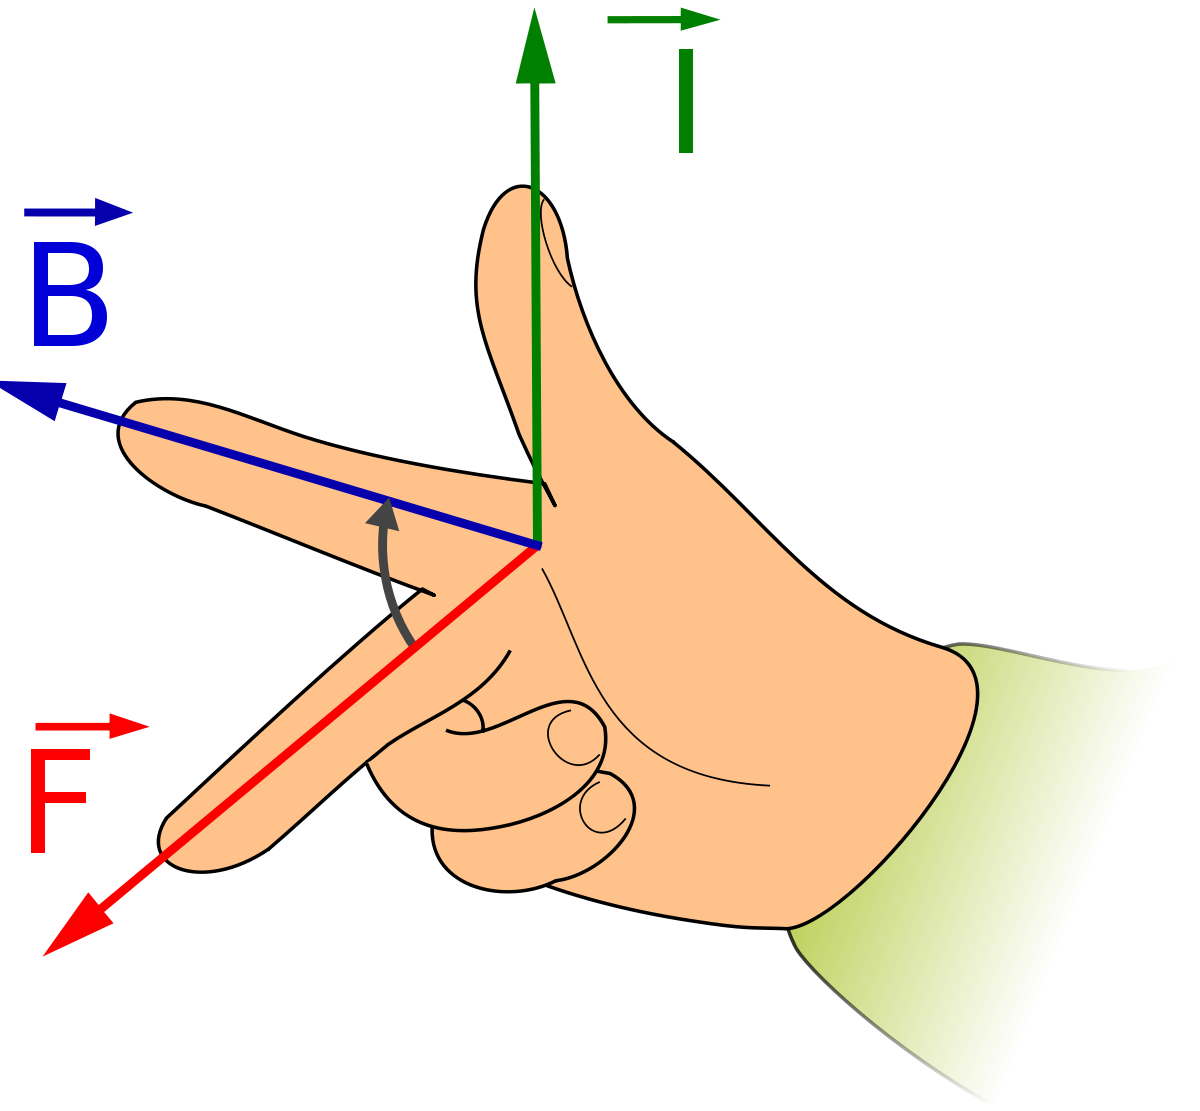
\includegraphics[width = \linewidth]{src/images/rechte_hand_lorenz.png}
    \end{minipage}
    \begin{minipage}{0.49\linewidth}
        \begin{scriptsize}
            \begin{empheq}{align*}
                l = &\text{Länge stromdurchflossener}\\
                &\text{Leiter in Magnetfeld}\\
                A = &\text{Querschnittsfläche Leiter}\\
                V = &A \cdot l = \text{Volumen Leiter}\\
                j = &\frac{I}{A} = \text{Flächenstromdichte}\\
                \rho = &\text{Volumenladungsdichte}\\
                \overrightarrow{B} = &\text{Magnetfeld}\\
                I = &\rho A v = \text{el. Strom}\\
                v = &\text{Geschwindigkeit der Ladungen}\\
                q = &\text{Ladung !Vorzeichen!}
            \end{empheq}
            \linebreak
            ACHTUNG: Elektronenfluss in entgegengesetzte Richtung zu Fluss des technischen Stroms
        \end{scriptsize}
    \end{minipage}        
%
    \subsubsection{Beispiel Elektromotor}
        \begin{minipage}{0.54\linewidth}
            \begin{empheq}[box = \fbox]{align*}
                M &= I (\overrightarrow{A} \times \overrightarrow{B})\\
                M_{\text{dip}} &= \overrightarrow{m} \times \overrightarrow{B}\\
                W &= -\int M_{\text{dip}} d\alpha = \overrightarrow{m} \overrightarrow{B}
            \end{empheq}
            \begin{scriptsize}
                \begin{empheq}{align*}
                    \overrightarrow{A} &= \text{Vektor normal zu Fläche}\\
                    \overrightarrow{B} &= \text{mag. Flussdichte}\\
                    \overrightarrow{m} &= \text{mag. Dipolmoment}\\
                \end{empheq}
            \end{scriptsize}
        \end{minipage}
        \begin{minipage}{0.44\linewidth}
            "Kommutator" kehrt Polarisierung des Stroms nach halber Umdrehungen um, damit volle Umdrehung ermöglicht wird.
            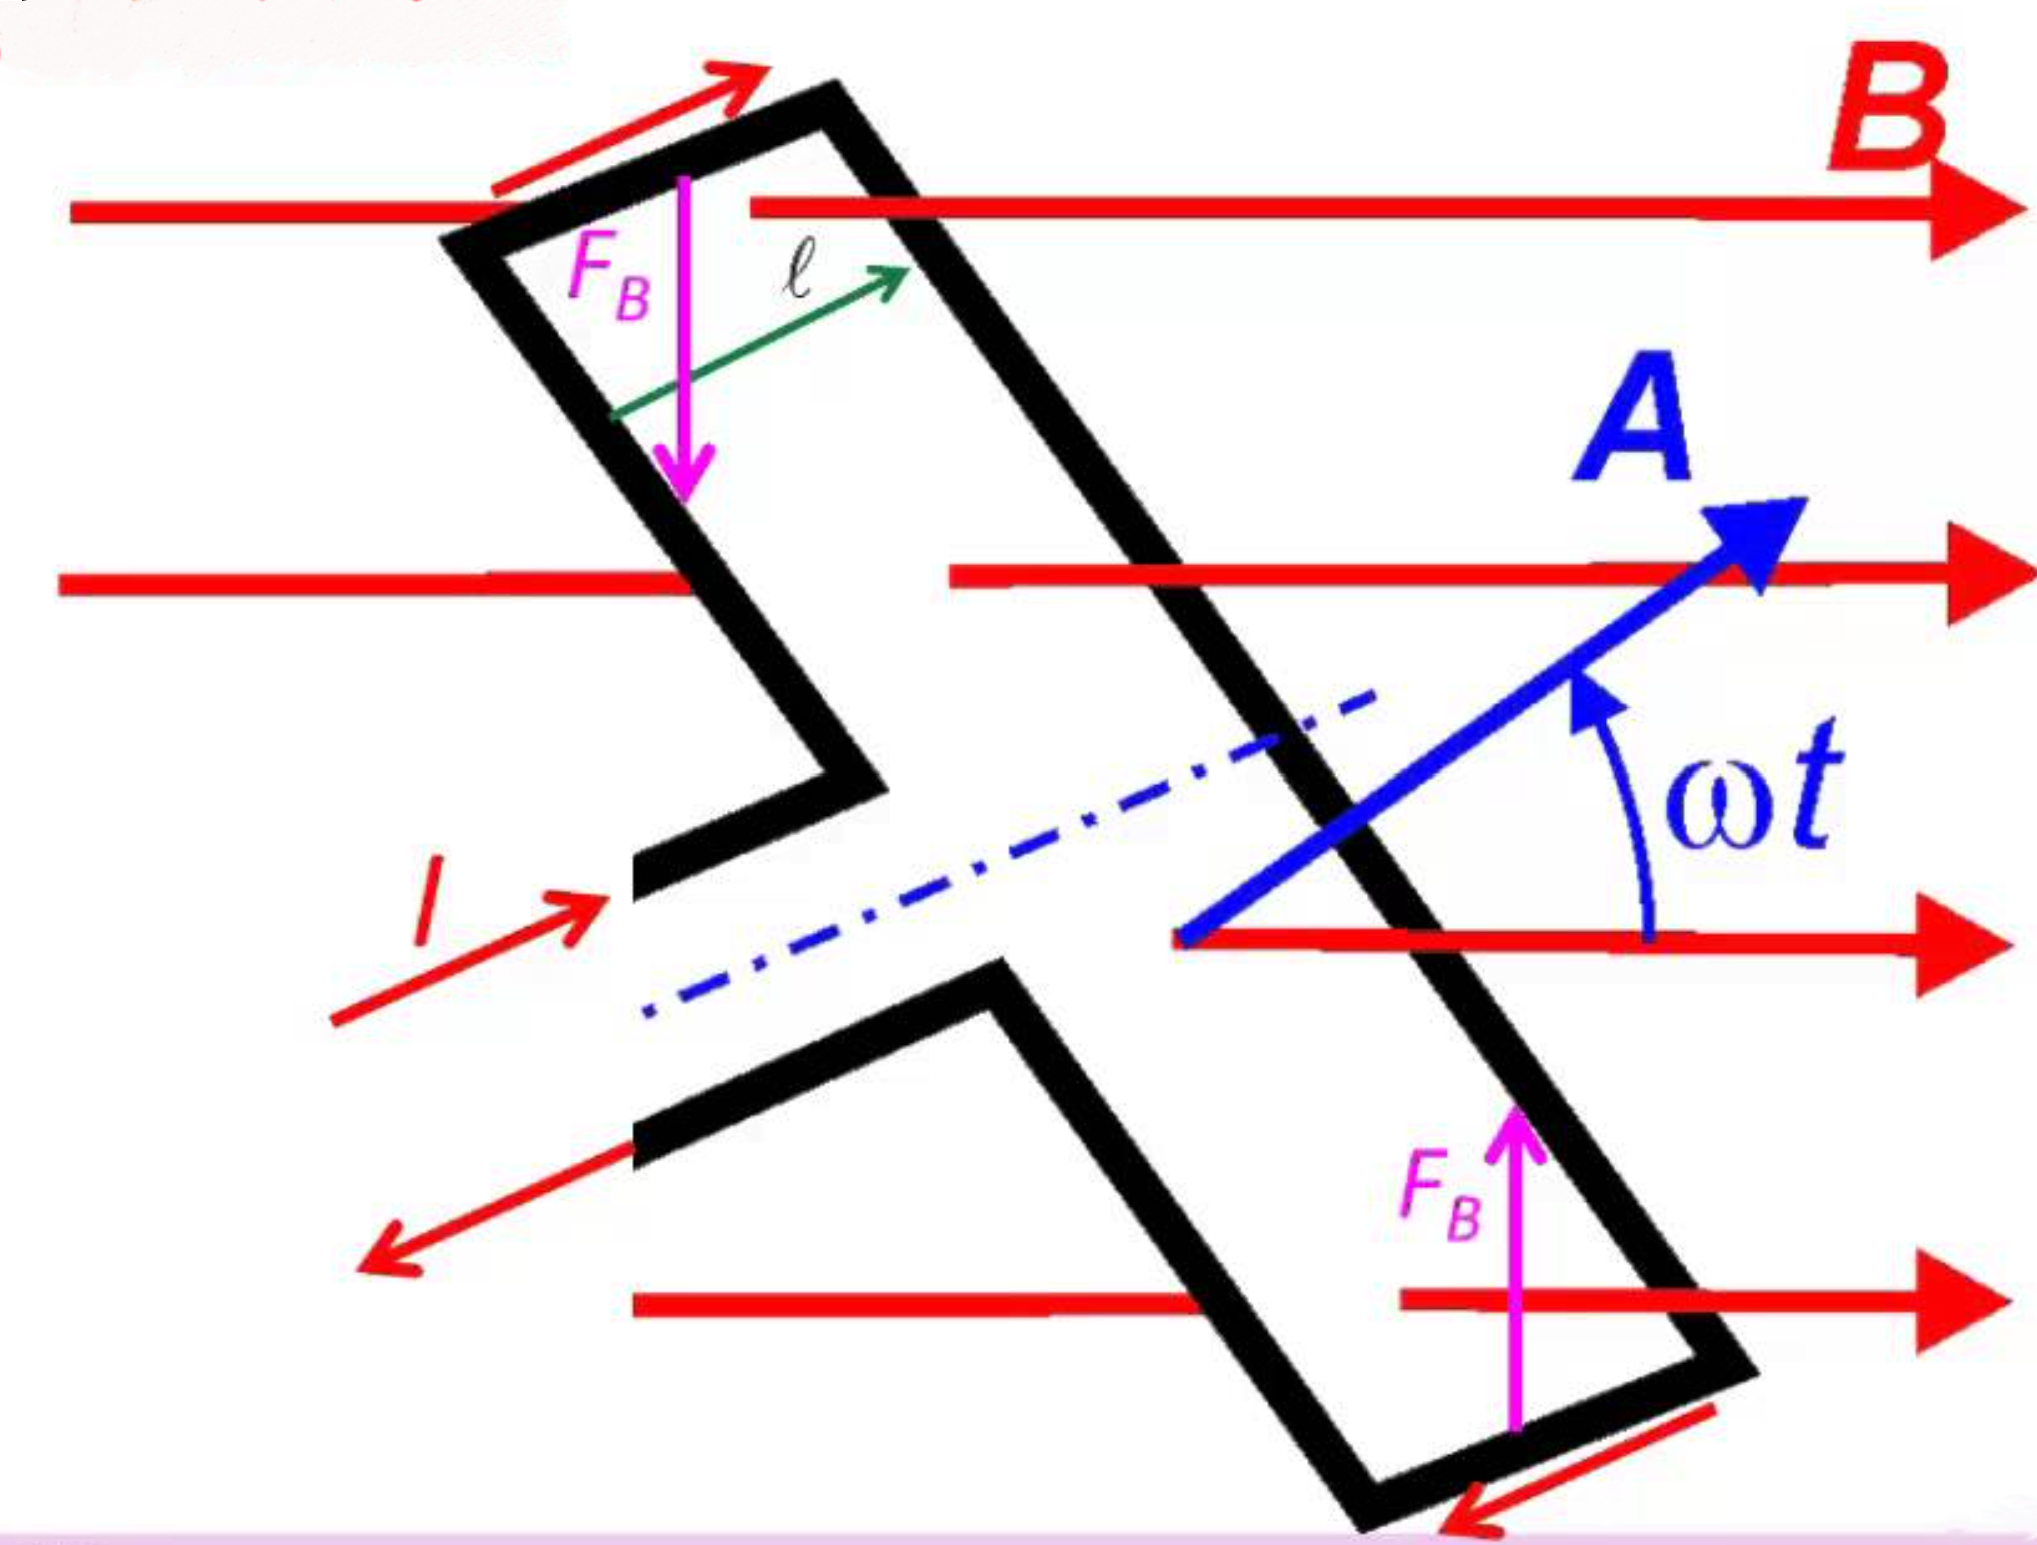
\includegraphics[width = \linewidth]{src/images/leiterschleife.png}
        \end{minipage}
%
    \subsubsection*{Beispiel parallele stromdurchflossene Drähte}
        \begin{minipage}{0.49\linewidth}
            \includegraphics*[width = \linewidth]{src/images/magnetische_wirkung_draehte.png}
        \end{minipage}
        \begin{minipage}{0.49\linewidth}
            \begin{itemize}
                \item $\overrightarrow{I_1} \uparrow \uparrow \overrightarrow{I_2}$: anziehend
                \item $\overrightarrow{I_1} \uparrow \downarrow \overrightarrow{I_2}$: abstossend
            \end{itemize}
            \mathbox{F_1 = F_2 = \frac{\mu_0}{2 \pi} l \frac{I_1 I_2}{r}}
        \end{minipage}
%
    \subsubsection*{Beispiel Leiterschleife verschiebbarer Bügel}